\documentclass[11pt,letterpaper]{article}
\usepackage[T1]{fontenc}
\usepackage{lmodern}
\usepackage[margin=1in]{geometry}
\usepackage{amsmath,amssymb,amsthm,mathtools}
\usepackage{enumitem}
\usepackage{microtype}
\usepackage{xcolor}
\usepackage{tikz}
\usepackage[colorlinks=true,linkcolor=blue,citecolor=blue,urlcolor=blue]{hyperref}
\usepackage{bookmark}
\pdftrailerid{}
\pdfsuppressptexinfo=15

\newtheorem{theorem}{Theorem}[section]
\newtheorem{proposition}[theorem]{Proposition}
\newtheorem{lemma}[theorem]{Lemma}
\newtheorem{corollary}[theorem]{Corollary}
\theoremstyle{definition}
\newtheorem{definition}[theorem]{Definition}
\theoremstyle{remark}
\newtheorem{remark}[theorem]{Remark}
\numberwithin{equation}{section}
\setlist{itemsep=3pt,topsep=5pt}
\hypersetup{pdftitle={Talagrand's discrete-convexity conjecture},
  pdfauthor={OpenAI},
  pdfsubject={A positive solution to Talagrand's Research Problem 13.3.2}}

\newcommand{\unverified}[1]{\par\smallskip\noindent\fbox{\parbox{0.95\linewidth}{\textbf{Unverified step.} #1}}\par\smallskip}
\newcommand{\step}[1]{\par\medskip\noindent\textbf{#1}\ }

\title{Talagrand's discrete-convexity conjecture}
\author{Rewritten for readability from the OpenAI manuscript of the same title}
\date{September 23, 2026}

\AddToHook{cmd/thebibliography/after}{\addcontentsline{toc}{section}{\refname}}

\begin{document}
\maketitle
\begin{abstract}
We prove Talagrand's discrete-convexity conjecture.
There is a universal integer $k$ (namely $k=2^{75}$) such that, whenever an
arbitrary family $\mathcal D$ of subsets of $\{1,\ldots,N\}$ has Bernoulli
product measure $\mu_p(\mathcal D)\ge 1-1/k$, the sets not contained in a
union of $k$ members of $\mathcal D$ admit a cover of total cost at most
$1/2$ at the same density $p$.
\end{abstract}

\section{The result and the shape of its proof}
\label{sec:introduction}

\subsection{Setting and statement}

Let $N\ge1$ and $[N]=\{1,\ldots,N\}$. We identify a subset of $[N]$ with its
indicator vector in $\{0,1\}^N$ whenever convenient. For $p\in(0,1)$,
$\mu_p$ is the probability measure on $2^{[N]}$ under which each coordinate
is present independently with probability $p$; that is,
$\mu_p(\{S\})=p^{|S|}(1-p)^{N-|S|}$.

\begin{definition}\label{def:basic}
Let $\mathcal D,\mathcal A,\mathcal G\subseteq 2^{[N]}$, let $k\ge1$ be an
integer, and let $\rho\in(0,1)$.
\begin{enumerate}[label=(\alph*)]
\item The \emph{exceptional family} is
\begin{equation}
\label{eq:exceptional-definition}
E_k(\mathcal D)
=\bigl\{S\subseteq[N]:
  S\nsubseteq D_1\cup\cdots\cup D_k
  \text{ for all }D_1,\ldots,D_k\in\mathcal D\bigr\}.
\end{equation}
The members $D_1,\ldots,D_k$ may repeat and need not be disjoint.
\item $\mathcal G$ \emph{covers} $\mathcal A$ if every $S\in\mathcal A$
contains some $I\in\mathcal G$. The members of $\mathcal G$ are called
\emph{generators}.
\item The \emph{cost} of $\mathcal G$ at density $\rho$ is
$c_\rho(\mathcal G)=\sum_{I\in\mathcal G}\rho^{|I|}$.
\item $\mathcal A$ is \emph{$\rho$-small} if it has a cover $\mathcal G$
with $c_\rho(\mathcal G)\le 1/2$.
\end{enumerate}
The same words are used with a finite ground set $X$ in place of $[N]$.
\end{definition}

Three immediate facts are used repeatedly.
\begin{enumerate}[label=(O\arabic*)]
\item\label{O:sub} \emph{Subadditivity.}
$c_\rho(\mathcal G\cup\mathcal G')\le c_\rho(\mathcal G)+c_\rho(\mathcal G')$.
If $\mathcal G$ covers $\mathcal A$ and $\mathcal G'$ covers $\mathcal A'$,
then $\mathcal G\cup\mathcal G'$ covers $\mathcal A\cup\mathcal A'$. A cover
of $\mathcal A$ covers every subfamily of $\mathcal A$. The empty family
covers the empty family at cost $0$.
\item\label{O:mono} \emph{Monotonicity in the density.} If
$\rho\le\rho'$ then $c_\rho(\mathcal G)\le c_{\rho'}(\mathcal G)$. Hence
$\rho'$-small implies $\rho$-small: smallness at a \emph{larger} density is
the \emph{stronger} property.
\item\label{O:union} \emph{Smallness bounds the measure.} Since
$\mu_p\{S:I\subseteq S\}=p^{|I|}$, a cover $\mathcal G$ of $\mathcal A$
gives $\mu_p(\mathcal A)\le\sum_{I\in\mathcal G}p^{|I|}=c_p(\mathcal G)$
by a union bound. So a $p$-small family has $\mu_p$-measure at most $1/2$,
with an explicit witness.
\end{enumerate}

\begin{theorem}[Main theorem]
\label{thm:main}
Set $k=2^{75}$. For every integer $N\ge1$, every $p\in(0,1)$, and every
family $\mathcal D\subseteq2^{[N]}$,
\[
\mu_p(\mathcal D)\ge1-\frac1k
\quad\Longrightarrow\quad
E_k(\mathcal D)\text{ is }p\text{-small}.
\]
\end{theorem}

The constant $k$ is independent of $N$, $p$, and $\mathcal D$. The family
$\mathcal D$ is arbitrary; no monotonicity is assumed.

\emph{Example.} If $\mathcal D=\{D:|D|\le d\}$, then
$E_k(\mathcal D)=\{S:|S|>kd\}$: a set lies in a union of $k$ sets of size at
most $d$ exactly when its size is at most $kd$. The theorem asserts that,
once $|D|\le d$ has probability at least $1-1/k$, the event $|S|>kd$ is not
only unlikely but has a cheap family of containment witnesses.

\subsection{Proof at a glance}
\label{sec:glance}

The proof has two layers and one combinatorial tool.

\paragraph{Outer layer: recovering the density (Section~\ref{sec:density}).}
Proposition~\ref{prop:half-density} is a version of the theorem that loses a
constant factor $L=2^{70}$ in the density: if $\mu_q(\mathcal F)\ge1/2$,
then $E_{32}(\mathcal F)$ is $(q/L)$-small. To get back to density $p$ we
apply it at the larger density $q=Lp$. We build, on one probability space,
$L$ random sets $R_1,\ldots,R_L$ that each have law $\mu_p$ but are
pairwise disjoint, so that their union has law $\mu_{Lp}$. Let $\mathcal F$
be the family of all unions of $L$ members of $\mathcal D$. A union bound
over the $L$ rows gives $\mu_{Lp}(\mathcal F)\ge1-L/k=31/32$, and
$E_{32}(\mathcal F)=E_{32L}(\mathcal D)=E_k(\mathcal D)$. The proposition
then gives smallness at density $Lp/L=p$. When $Lp\ge1$, a second coupling
shows directly that $E_k(\mathcal D)=\varnothing$.

\paragraph{Inner layer: a cover at density $q/L$ (Section~\ref{sec:weights}).}
Write $f=\mathbf 1_{\mathcal F}$. To each $U\subseteq[N]$ we attach a
weight $w(U)=b(U)^2\ge0$, a rescaled squared biased Fourier coefficient of
$f$. Two facts drive the argument.
\begin{itemize}
\item \emph{Global bound} (Lemma~\ref{lem:global}, by Parseval):
$\sum_{U}q^{|U|}w(U)\le1$.
\item \emph{Lower bound on exceptional sets} (Lemma~\ref{lem:exceptional},
by a signed product measure on $32\times N$ arrays): every
$S\in E_{32}(\mathcal F)$ satisfies
$\sum_{\varnothing\ne U\subseteq S}w(U)^{16}\ge2^{-32}$.
\end{itemize}
The cover is built as follows. Sets $U$ with $w(U)\ge2^{-64|U|}$ are taken
as generators; the global bound makes this cheap. The remaining sets are
sorted into bins $\mathcal H_{r,h}$ by size $r$ and dyadic weight
$w(U)\approx2^{-h}$, where necessarily $h\ge64r$. The global bound limits
the size of each bin, and the covering lemma gives a cheap cover of all sets
containing at least $2^{12h}$ members of the bin. A set $S$ containing no
generator contains fewer than $2^{12h}$ members of each bin, so its sum of
sixteenth powers is at most $\sum_{r,h}2^{12h}\cdot2^{-16h}<2^{-32}$; by the
lower bound, $S$ is not exceptional.

\paragraph{The tool: a covering lemma (Section~\ref{sec:covering}).}
Lemma~\ref{lem:covering} says: if a family $\mathcal H$ of $r$-sets has
$|\mathcal H|\rho^r\le2^{h+1}$, then the sets containing at least $2^{12h}$
members of $\mathcal H$ have a cover of cost at most $3\cdot2^{-h}$. The
cover is random and has three parts: small sets lying in unusually many
edges; unions of randomly sampled pairs of edges; and unions of those long
tuples of edges none of whose pairs was sampled. A long tuple has
quadratically many pairs, so it is very unlikely to survive.

\begin{center}
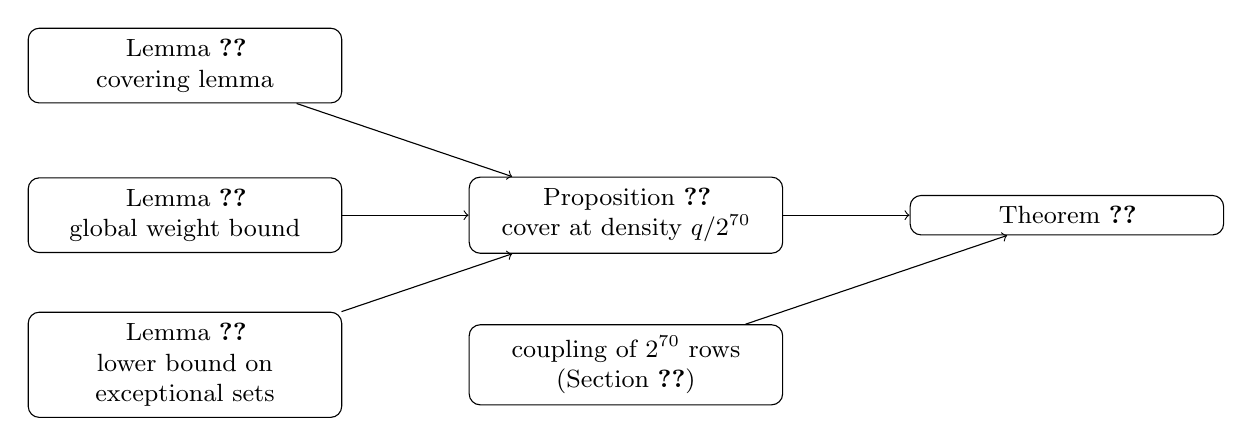
\begin{tikzpicture}[
  box/.style={draw,rounded corners,align=center,inner sep=4pt,
              text width=3.7cm,font=\small}]
  \node[box] (cov) at (0,1.9)
    {Lemma~\ref{lem:covering}\\ covering lemma};
  \node[box] (glob) at (0,0)
    {Lemma~\ref{lem:global}\\ global weight bound};
  \node[box] (exc) at (0,-1.9)
    {Lemma~\ref{lem:exceptional}\\ lower bound on exceptional sets};
  \node[box] (prop) at (5.6,0)
    {Proposition~\ref{prop:half-density}\\ cover at density $q/2^{70}$};
  \node[box] (coup) at (5.6,-1.9)
    {coupling of $2^{70}$ rows\\ (Section~\ref{sec:density})};
  \node[box] (thm) at (11.2,0)
    {Theorem~\ref{thm:main}};
  \draw[->] (cov) -- (prop);
  \draw[->] (glob) -- (prop);
  \draw[->] (exc) -- (prop);
  \draw[->] (prop) -- (thm);
  \draw[->] (coup) -- (thm);
\end{tikzpicture}
\end{center}

Sections~\ref{sec:covering}, \ref{sec:weights} and~\ref{sec:density} are
self-contained apart from Parseval's identity. Section~\ref{sec:context}
collects a consequence, the context, and a side result
(Corollary~\ref{cor:two-union}) that is \emph{not} used in the proof of
Theorem~\ref{thm:main} and that rests on cited results.

\subsection{Notation changes relative to the source}

To keep one meaning per symbol, a few letters of the source are renamed.
In Lemma~\ref{lem:covering}: the degree threshold is $\tau$ (source: $T$)
and the length of a partial tuple is $n$ (source: $t$). In
Section~\ref{sec:weights}: a $\mu_q$-random point is $\xi$ (source: $X$),
a $32\times N$ array is $A$ (source: $x$), and the signed column mass is
$\widetilde P$ (source: $R$). In Section~\ref{sec:density}: the conditional
inclusion probability is $\theta$ (source: $t$). In
Corollary~\ref{cor:two-union}: the intermediate density is $p_1$
(source: $r$). The mathematics is unchanged.

\section{An elementary covering lemma}
\label{sec:covering}

\begin{lemma}[Covering lemma]\label{lem:covering}
Let \(X\) be a finite set, let \(0<\rho<1\), and let \(r,h\) be integers
with \(1\le r\le h\) and \(h\ge64\). Suppose that
\(\mathcal H\subseteq\binom{X}{r}\) (a family of $r$-element subsets of $X$,
called \emph{edges}) satisfies
\[
|\mathcal H|\rho^r\le2^{h+1}.
\]
Then the family
\[
\mathcal M=\left\{S\subseteq X:
  |\{e\in\mathcal H:e\subseteq S\}|\ge2^{12h}\right\}
\]
has a cover \(\mathcal G\subseteq2^X\) with
\(c_\rho(\mathcal G)\le3\cdot2^{-h}\).
\end{lemma}

\emph{Where it is used.} Once for each occupied bin in Step~3 of the proof
of Proposition~\ref{prop:half-density}, with $X=[N]$, $\rho=q/2^{70}$ and
$\mathcal H=\mathcal H_{r,h}$.

\emph{Plan.} We build a random family
$\mathcal G=\mathcal C_0\cup\mathcal C_1\cup\mathcal C_2$ that covers
$\mathcal M$ for \emph{every} outcome of the randomness, and show that its
\emph{expected} cost is at most $3\cdot2^{-h}$; some outcome then does at
least as well. $\mathcal C_0$ is deterministic and its cost is bounded by
double counting (Steps~1--2). Removing $\mathcal C_0$ leaves ``regular''
edges with a uniform extension bound (Step~3), which controls the costs of
$\mathcal C_1$ (Step~4) and $\mathcal C_2$ (Steps~5--8).

\begin{proof}
Fix the parameters
\[
m=2^{12h},\qquad \tau=2^{4h},\qquad \pi=2^{-6h},
\]
where $\pi$ is a probability, not the circle constant. Note
$\pi m=2^{6h}$.

\step{Step 1 (weighted degrees and a double count).}
For \(I\subseteq X\) with \(|I|\le r\), define the \emph{weighted degree}
\[
d(I)=|\{e\in\mathcal H:I\subseteq e\}|\,\rho^{r-|I|}.
\]
Then
\begin{equation}\label{eq:double-count}
\sum_{\substack{I\subseteq X\\|I|\le r}}d(I)\rho^{|I|}
=\rho^r\sum_{\substack{I\subseteq X\\|I|\le r}}
   |\{e\in\mathcal H:I\subseteq e\}|
=\rho^r\sum_{e\in\mathcal H}|\{I:I\subseteq e\}|
=2^r|\mathcal H|\rho^r .
\end{equation}
The middle equality exchanges the order of summation over pairs $(I,e)$
with $I\subseteq e$; every subset of an edge has size at most $r$, and an
edge has $2^r$ subsets.

\step{Step 2 (high-degree generators $\mathcal C_0$).}
Let
\[
\mathcal C_0=\{I\subseteq X:|I|\le r,\ d(I)>\tau\}.
\]
For $I\in\mathcal C_0$ we have $\rho^{|I|}<\tau^{-1}d(I)\rho^{|I|}$.
Summing over $\mathcal C_0$, enlarging the sum to all $I$ with $|I|\le r$
(the terms are nonnegative), and using \eqref{eq:double-count}, the
hypothesis $|\mathcal H|\rho^r\le2^{h+1}$, and $r\le h$:
\begin{equation}\label{eq:covering-initial-cost}
c_\rho(\mathcal C_0)
\le \tau^{-1}2^r|\mathcal H|\rho^r
\le 2^{-4h}\cdot2^{r}\cdot2^{h+1}
=2^{r+1-3h}\le2^{1-2h}.
\end{equation}

\step{Step 3 (regular edges and the extension bound).}
Call an edge \emph{regular} if it contains no member of \(\mathcal C_0\),
and let \(\mathcal H'\subseteq\mathcal H\) be the family of regular edges.
If $I\subseteq e$ for some $e\in\mathcal H'$, then $|I|\le r$ and
$I\notin\mathcal C_0$, so
\begin{equation}\label{eq:regular}
I\subseteq e\in\mathcal H'
\quad\Longrightarrow\quad d(I)\le \tau.
\end{equation}
\emph{Claim.} For every \(B\subseteq X\),
\begin{equation}\label{eq:covering-extension}
\sum_{e\in\mathcal H'}\rho^{|e\setminus B|}
\le \tau\sum_{i=0}^r\binom{|B|}{i}.
\end{equation}
\emph{Proof of the claim.} Group the edges \(e\in\mathcal H'\) according to
the set \(I=e\cap B\). If the group of $I$ is nonempty, then $I\subseteq B$,
$|I|\le r$, every edge $e$ in the group has $|e\setminus B|=r-|I|$, and
$d(I)\le\tau$ by \eqref{eq:regular}. Hence the group contributes
\[
\sum_{\substack{e\in\mathcal H'\\e\cap B=I}}
  \rho^{|e\setminus B|}
=|\{e\in\mathcal H':e\cap B=I\}|\,\rho^{r-|I|}
\le|\{e\in\mathcal H:I\subseteq e\}|\,\rho^{r-|I|}
= d(I)\le \tau.
\]
The number of groups is at most the number of subsets of $B$ of size at most
$r$, which is $\sum_{i=0}^r\binom{|B|}{i}$. This proves
\eqref{eq:covering-extension}.

\step{Step 4 (sampled pairs $\mathcal C_1$).}
For each ordered pair \((e,e')\in(\mathcal H')^2\), diagonal pairs
included, let $\sigma(e,e')\in\{0,1\}$ be independent random variables with
$\mathbb P(\sigma(e,e')=1)=\pi$. A pair with $\sigma(e,e')=1$ is called
\emph{sampled}. Let
\[
\mathcal C_1=\{e\cup e':(e,e')\in(\mathcal H')^2,\ \sigma(e,e')=1\}.
\]
Several pairs may have the same union, which is counted once in
$c_\rho(\mathcal C_1)$; therefore
$c_\rho(\mathcal C_1)\le\sum_{e,e'}\sigma(e,e')\rho^{|e\cup e'|}$.
Applying \eqref{eq:covering-extension} with \(B=e\), so that \(|B|=r\) and
$\sum_{i=0}^r\binom ri=2^r$, gives
$\sum_{e'\in\mathcal H'}\rho^{|e'\setminus e|}\le2^r\tau$. Since
$|e\cup e'|=r+|e'\setminus e|$,
\begin{align}
\mathbb E[c_\rho(\mathcal C_1)]
&\le\pi\sum_{e\in\mathcal H'}\rho^{r}
    \sum_{e'\in\mathcal H'}\rho^{|e'\setminus e|}
\le\pi\,|\mathcal H'|\rho^r\,2^r\tau
\notag\\
&\le2^{-6h}\cdot2^{h+1}\cdot2^{r}\cdot2^{4h}
=2^{r+1-3h}\le2^{1-2h}.
\label{eq:covering-pair-cost}
\end{align}
Here we used $|\mathcal H'|\rho^r\le|\mathcal H|\rho^r\le2^{h+1}$ and
$r\le h$.

\step{Step 5 (residual generators $\mathcal C_2$; the cover).}
Call an ordered tuple \((e_1,\ldots,e_m)\) of \emph{distinct} regular
edges \emph{unsampled} if $\sigma(e_i,e_j)=0$ for all $1\le i,j\le m$. Let
\[
\mathcal C_2=\{e_1\cup\cdots\cup e_m:
 (e_1,\ldots,e_m)\text{ an unsampled tuple of distinct regular edges}\},
\qquad
\mathcal G=\mathcal C_0\cup\mathcal C_1\cup\mathcal C_2 .
\]
\emph{Claim: $\mathcal G$ covers $\mathcal M$ for every outcome of
$\sigma$.} Let $S\in\mathcal M$. If $S$ contains a member of
$\mathcal C_0$ we are done. Otherwise every edge $e\subseteq S$ is regular
(a member of $\mathcal C_0$ inside $e$ would lie inside $S$), so $S$
contains at least $m$ distinct regular edges; choose $m$ of them,
$e_1,\ldots,e_m$. If some pair $(e_i,e_j)$ is sampled, then
$e_i\cup e_j\in\mathcal C_1$ and $e_i\cup e_j\subseteq S$. If no pair is
sampled, then $e_1\cup\cdots\cup e_m\in\mathcal C_2$ and it is contained in
$S$.

\step{Step 6 (total weight of tuples).}
For \(0\le n\le m\), let
\[
W_n=
\sum_{\substack{(e_1,\ldots,e_n)\in(\mathcal H')^n\\
                e_1,\ldots,e_n\ \text{distinct}}}
  \rho^{|e_1\cup\cdots\cup e_n|},
\qquad W_0=1.
\]
\emph{Claim: $W_{n+1}\le \tau(1+rm)^r\,W_n$ for $0\le n<m$, hence
$W_m\le[\tau(1+rm)^r]^m$.}
Fix a tuple $(e_1,\ldots,e_n)$ of distinct regular edges with union $B$;
then $|B|\le rn\le rm$. Each way of extending it by a further edge
$e\in\mathcal H'$ has weight
$\rho^{|B\cup e|}=\rho^{|B|}\rho^{|e\setminus B|}$. Summing over
\emph{all} $e\in\mathcal H'$ (dropping the requirement that $e$ differ from
$e_1,\ldots,e_n$ only adds nonnegative terms) and using
\eqref{eq:covering-extension},
\[
\sum_{e\in\mathcal H'}\rho^{|B\cup e|}
\le\rho^{|B|}\,\tau\sum_{i=0}^r\binom{|B|}{i}
\le\rho^{|B|}\,\tau(1+|B|)^r
\le\rho^{|B|}\,\tau(1+rm)^r .
\]
The middle inequality $\sum_{i=0}^r\binom{|B|}{i}\le(1+|B|)^r$ holds
because the map sending a subset $\{x_1<\cdots<x_i\}$ of $B$ (with respect
to a fixed order of $B$, $i\le r$) to the sequence
$(x_1,\ldots,x_i,\ast,\ldots,\ast)$ of length $r$ over the alphabet
$B\cup\{\ast\}$ is injective. Summing over all tuples $(e_1,\ldots,e_n)$
gives the claim, and iterating from $W_0=1$ gives the bound on $W_m$.

\step{Step 7 (expected cost of $\mathcal C_2$).}
Fix a tuple $(e_1,\ldots,e_m)$ of distinct regular edges. Because the
edges are distinct, the $m^2$ ordered pairs $(e_i,e_j)$ are $m^2$
\emph{distinct} elements of $(\mathcal H')^2$, so the corresponding
variables $\sigma(e_i,e_j)$ are independent and
\[
\mathbb P\bigl((e_1,\ldots,e_m)\text{ is unsampled}\bigr)
=(1-\pi)^{m^2}\le\exp(-\pi m^2)\le2^{-\pi m^2},
\]
using $1-\pi\le\exp(-\pi)$ and $\exp(1)>2$. Each member of $\mathcal C_2$
is the union of at least one unsampled tuple, so $c_\rho(\mathcal C_2)$ is
at most the sum of $\rho^{|e_1\cup\cdots\cup e_m|}$ over unsampled tuples.
By linearity of expectation and Step~6,
\[
\mathbb E[c_\rho(\mathcal C_2)]
\le W_m\,(1-\pi)^{m^2}
\le[\tau(1+rm)^r]^m\,2^{-\pi m^2}.
\]

\step{Step 8 (numerics).}
We show the last bound is at most $2^{-m}$. Taking $\log_2$ and dividing by
$m$, it suffices that
\[
\log_2 \tau+r\log_2(1+rm)+1\le\pi m=2^{6h}.
\]
Using $r\le h$ and $h+1\le2^h$,
\[
1+rm\le1+h\,2^{12h}\le(h+1)2^{12h}\le2^{13h},
\]
so the left side is at most $4h+13rh+1\le4h+13h^2+1\le18h^2$ (as
$4h+1\le5h^2$ for $h\ge1$). Finally $h\le 2^h$ gives
$18h^2\le18\cdot2^{2h}\le2^{6h}$, the last step because $18\le2^{4h}$
(true for $h\ge3$, in particular for $h\ge64$). Therefore
\begin{equation}\label{eq:covering-residual-cost}
\mathbb E[c_\rho(\mathcal C_2)]
\le2^{(4h+13rh)m-\pi m^2}\le2^{-m}.
\end{equation}

\step{Step 9 (conclusion).}
By subadditivity \ref{O:sub} and
\eqref{eq:covering-initial-cost}, \eqref{eq:covering-pair-cost},
\eqref{eq:covering-residual-cost},
\[
\mathbb E[c_\rho(\mathcal G)]
\le2^{1-2h}+2^{1-2h}+2^{-m}
=2^{2-2h}+2^{-m}\le 2^{-h}+2^{-h}\le3\cdot2^{-h},
\]
where $2^{2-2h}\le2^{-h}$ because $h\ge2$, and $2^{-m}\le2^{-h}$ because
$m=2^{12h}\ge h$. The sample space $\{0,1\}^{(\mathcal H')^2}$ is finite,
so some outcome of $\sigma$ has $c_\rho(\mathcal G)$ at most its
expectation. By Step~5 that outcome gives a cover of $\mathcal M$.
\end{proof}

\section{Weights for exceptional sets}
\label{sec:weights}

This section proves the fixed-loss version of the main theorem.

\begin{proposition}\label{prop:half-density}
Let $L=2^{70}$. For every integer $N\ge1$, every $q\in(0,1)$, and every
$\mathcal F\subseteq 2^{[N]}$ satisfying $\mu_q(\mathcal F)\ge1/2$,
the family $E_{32}(\mathcal F)$ is $(q/L)$-small.
\end{proposition}

\emph{Where it is used.} In Case~1 of the proof of Theorem~\ref{thm:main},
with $q=Lp$.

Throughout this section $N$, $q$ and $\mathcal F$ are fixed, and
$f=\mathbf 1_{\mathcal F}\colon\{0,1\}^N\to\{0,1\}$.

\begin{definition}[Weights]\label{def:weights}
For $U\subseteq[N]$, $z\in\{0,1\}^U$ and $y\in\{0,1\}^{[N]\setminus U}$,
write $(z,y)\in\{0,1\}^N$ for the vector equal to $z$ on $U$ and to $y$
off $U$. Let $Y$ be a random vector with independent Bernoulli-$q$
coordinates indexed by $[N]\setminus U$. Define
\begin{equation}\label{eq:weights-definition}
 b(U)=(1-q)^{|U|}
 \sum_{z\in\{0,1\}^{U}}(-1)^{\sum_{i\in U}z_i}\,
 \mathbb E[f(z,Y)],
 \qquad w(U)=b(U)^2 .
\end{equation}
\end{definition}

For $U=\varnothing$ the sum has one term and $Y$ is a full $\mu_q$-sample,
so
\begin{equation}\label{eq:b-empty}
b(\varnothing)=\mathbb E[f(Y)]=\mu_q(\mathcal F).
\end{equation}
As a further illustration,
$b(\{i\})=(1-q)\bigl(\mathbb E[f(0,Y)]-\mathbb E[f(1,Y)]\bigr)$.

\subsection{The global weight bound}

\begin{lemma}[Global weight bound]\label{lem:global}
For every $q\in(0,1)$ and every $\mathcal F\subseteq2^{[N]}$,
\begin{equation}\label{eq:global-weight-bound}
 \sum_{U\subseteq[N]}q^{|U|}w(U)\le\mu_q(\mathcal F)\le1 .
\end{equation}
\end{lemma}

\emph{Where it is used.} Steps~1 and~2 of the proof of
Proposition~\ref{prop:half-density}.

\emph{Plan.} Identify $b(U)$ with a biased Fourier coefficient of $f$ up to
an explicit factor, then apply Parseval. The basis is the standard biased
Fourier basis \cite[Section~8.4]{ODonnell14}; its normalization is made
explicit here.

\begin{proof}
Let $\xi=(\xi_1,\ldots,\xi_N)\sim\mu_q$.

\step{Step 1 (an orthonormal basis).}
For $i\in[N]$ put $g_i(x)=(q-x_i)/\sqrt{q(1-q)}$ and, for
$U\subseteq[N]$,
\[
 \chi_U(x)=\prod_{i\in U}g_i(x)
 =\frac{\prod_{i\in U}(q-x_i)}{[q(1-q)]^{|U|/2}} .
\]
Since $\mathbb E\xi_i=q$ and $\operatorname{Var}\xi_i=q(1-q)$, we have
$\mathbb E[g_i(\xi)]=0$ and $\mathbb E[g_i(\xi)^2]=1$. For
$U,V\subseteq[N]$, independence of the coordinates gives
\[
\mathbb E[\chi_U(\xi)\chi_V(\xi)]
=\prod_{i\in U\cap V}\mathbb E[g_i(\xi)^2]
 \prod_{i\in U\triangle V}\mathbb E[g_i(\xi)]
=\begin{cases}1,&U=V,\\0,&U\ne V.\end{cases}
\]
Because $0<q<1$, $\mu_q$ has full support, so
$\langle g,g'\rangle=\mathbb E[g(\xi)g'(\xi)]$ is an inner product on the
$2^N$-dimensional space of real functions on $\{0,1\}^N$. The $2^N$
functions $\chi_U$ are orthonormal, hence a basis. With
$\widehat f(U)=\mathbb E[f(\xi)\chi_U(\xi)]$, Parseval's identity reads
\begin{equation}\label{eq:parseval}
\sum_{U\subseteq[N]}\widehat f(U)^2=\mathbb E[f(\xi)^2].
\end{equation}

\step{Step 2 (relation between $\widehat f$ and $b$).}
We claim
\begin{equation}\label{eq:fhat-b}
 \widehat f(U)=\left(\frac{q}{1-q}\right)^{|U|/2}b(U).
\end{equation}
For one Bernoulli-$q$ bit and $z_i\in\{0,1\}$,
\[
 \mathbb P(\xi_i=z_i)\,(q-z_i)=q(1-q)(-1)^{z_i},
\]
since for $z_i=0$ the left side is $(1-q)q$ and for $z_i=1$ it is
$q(q-1)$. Conditioning on the coordinates of $\xi$ in $U$ (the remaining
coordinates have the law of $Y$ and are independent of them),
\begin{align*}
\widehat f(U)
&=\sum_{z\in\{0,1\}^U}
  \frac{\prod_{i\in U}\mathbb P(\xi_i=z_i)(q-z_i)}{[q(1-q)]^{|U|/2}}\,
  \mathbb E[f(z,Y)]
 =[q(1-q)]^{|U|/2}
 \sum_{z\in\{0,1\}^{U}}(-1)^{\sum_{i\in U}z_i}\,\mathbb E[f(z,Y)]\\
&=[q(1-q)]^{|U|/2}(1-q)^{-|U|}\,b(U)
 =\left(\frac{q}{1-q}\right)^{|U|/2}b(U).
\end{align*}

\step{Step 3 (conclusion).}
Squaring \eqref{eq:fhat-b} gives
$q^{|U|}w(U)=(1-q)^{|U|}\widehat f(U)^2\le\widehat f(U)^2$. Summing over
$U$ and using \eqref{eq:parseval} and $f^2=f$,
\[
 \sum_{U\subseteq[N]}q^{|U|}w(U)
 \le\sum_{U\subseteq[N]}\widehat f(U)^2
 =\mathbb E[f(\xi)^2]
 =\mu_q(\mathcal F)\le1. \qedhere
\]
\end{proof}

\subsection{A lower bound on every exceptional set}

\begin{lemma}[Lower bound on exceptional sets]\label{lem:exceptional}
Assume $\mu_q(\mathcal F)\ge1/2$. Then every $S\in E_{32}(\mathcal F)$
satisfies
\begin{equation}\label{eq:exceptional-weight-bound}
 \sum_{\varnothing\ne U\subseteq S}w(U)^{16}\ge2^{-32}.
\end{equation}
\end{lemma}

\emph{Where it is used.} Step~5 of the proof of
Proposition~\ref{prop:half-density}.

\emph{Plan.} Put a signed product weight $\nu_S$ on $32\times N$ arrays of
bits so that (i) $\nu_S$ vanishes unless the $32$ rows, read as sets, have
union containing $S$, and (ii) $\nu_S$ is a sum of terms that factor
across the rows. Property (i) and $S\in E_{32}(\mathcal F)$ force
$\sum_A\nu_S(A)\prod_jf(\text{row }j)=0$; property (ii) evaluates this sum
as $\sum_{U\subseteq S}(-1)^{|U|}b(U)^{32}$. Isolating $U=\varnothing$
gives the bound.

\begin{proof}
Fix $S\in E_{32}(\mathcal F)$. An \emph{array} is
$A=(A_{ji})\in\{0,1\}^{32\times N}$; its $j$-th row is
$A_j=(A_{j1},\ldots,A_{jN})\in\{0,1\}^N$, and its $i$-th column is
$A^{(i)}=(A_{1i},\ldots,A_{32,i})\in\{0,1\}^{32}$.

\step{Step 1 (column masses).}
For a column $y\in\{0,1\}^{32}$ let
\[
 P(y)=\prod_{j=1}^{32}q^{y_j}(1-q)^{1-y_j},
 \qquad
 \widetilde P(y)=P(y)-(1-q)^{32}(-1)^{\sum_{j=1}^{32}y_j}.
\]
$P$ is the mass function of $32$ independent Bernoulli-$q$ bits, and
$\widetilde P$ is a signed modification with
\begin{equation}\label{eq:zero-column}
\widetilde P(0,\ldots,0)=(1-q)^{32}-(1-q)^{32}=0.
\end{equation}
Define the signed weight of an array by
\[
\nu_S(A)=\prod_{i\notin S}P(A^{(i)})\prod_{i\in S}\widetilde P(A^{(i)}).
\]

\step{Step 2 (a vanishing sum).}
We claim
\begin{equation}\label{eq:vanishing}
 \sum_{A\in\{0,1\}^{32\times N}}\nu_S(A)
 \prod_{j=1}^{32}f(A_j)=0 .
\end{equation}
Indeed, every term is zero. If $\nu_S(A)\ne0$, then by
\eqref{eq:zero-column} no column $A^{(i)}$ with $i\in S$ is all-zero, i.e.\
every $i\in S$ belongs to at least one of the sets $A_1,\ldots,A_{32}$, so
$S\subseteq A_1\cup\cdots\cup A_{32}$. As $S\in E_{32}(\mathcal F)$, the
rows cannot all lie in $\mathcal F$, so $\prod_jf(A_j)=0$. Only pointwise
vanishing is used; the signs of $\nu_S$ play no role.

\step{Step 3 (expanding the product over $S$).}
Expanding $\prod_{i\in S}\widetilde P(A^{(i)})$ and letting
$U\subseteq S$ be the set of columns where the subtracted term is chosen,
\[
\nu_S(A)=\sum_{U\subseteq S}(-1)^{|U|}\lambda_U(A),
\qquad
\lambda_U(A)=(1-q)^{32|U|}
\prod_{i\in U}(-1)^{\sum_{j=1}^{32}A_{ji}}
\prod_{i\notin U}P(A^{(i)}).
\]
(Columns outside $S$ and columns in $S\setminus U$ both carry $P$.)

\step{Step 4 (factoring over rows).}
Regroup the three factors of $\lambda_U(A)$ by rows:
\[
(1-q)^{32|U|}=\prod_{j=1}^{32}(1-q)^{|U|},\quad
\prod_{i\in U}(-1)^{\sum_{j}A_{ji}}
 =\prod_{j=1}^{32}(-1)^{\sum_{i\in U}A_{ji}},\quad
\prod_{i\notin U}P(A^{(i)})
 =\prod_{j=1}^{32}\prod_{i\notin U}q^{A_{ji}}(1-q)^{1-A_{ji}} .
\]
Hence $\lambda_U(A)=\prod_{j=1}^{32}\beta_U(A_j)$, where for
$x\in\{0,1\}^N$
\[
\beta_U(x)=(1-q)^{|U|}(-1)^{\sum_{i\in U}x_i}
\prod_{i\notin U}q^{x_i}(1-q)^{1-x_i}.
\]
Since the rows of $A$ range independently over $\{0,1\}^N$,
\[
\sum_{A}\lambda_U(A)\prod_{j=1}^{32}f(A_j)
=\Bigl(\sum_{x\in\{0,1\}^N}\beta_U(x)f(x)\Bigr)^{32}.
\]
Writing $x=(z,y)$ with $z\in\{0,1\}^U$ and
$y\in\{0,1\}^{[N]\setminus U}$, the product over $i\notin U$ is the
probability that $Y=y$, so
\[
\sum_{x}\beta_U(x)f(x)
=(1-q)^{|U|}\sum_{z\in\{0,1\}^U}(-1)^{\sum_{i\in U}z_i}\,
 \mathbb E[f(z,Y)]=b(U)
\]
by \eqref{eq:weights-definition}. Combining with Step~3 and
\eqref{eq:vanishing} (all sums are finite),
\begin{equation}\label{eq:signed-identity}
 0=\sum_{U\subseteq S}(-1)^{|U|}b(U)^{32}.
\end{equation}

\step{Step 5 (conclusion).}
The term $U=\varnothing$ in \eqref{eq:signed-identity} is
$b(\varnothing)^{32}=\mu_q(\mathcal F)^{32}\ge2^{-32}$ by
\eqref{eq:b-empty} and the hypothesis. Moving the other terms to the other
side and using the triangle inequality,
\[
 2^{-32}\le b(\varnothing)^{32}
 =-\sum_{\varnothing\ne U\subseteq S}(-1)^{|U|}b(U)^{32}
 \le\sum_{\varnothing\ne U\subseteq S}|b(U)|^{32}
 =\sum_{\varnothing\ne U\subseteq S}w(U)^{16}. \qedhere
\]
\end{proof}

\subsection{Proof of Proposition~\ref{prop:half-density}}

\emph{Plan.} Take heavy sets as generators (Step~1), sort the rest into
bins (Step~2), cover each bin's ``many members'' family by
Lemma~\ref{lem:covering} (Step~3), add up the costs (Step~4), and show via
Lemma~\ref{lem:exceptional} that a set containing no generator is not
exceptional (Step~5). The gap exploited is that fewer than $2^{12h}$ weights
of size at most $2^{-h}$ contribute less than
$2^{12h}\cdot2^{-16h}=2^{-4h}$ to a sum of sixteenth powers.

\begin{proof}[Proof of Proposition~\ref{prop:half-density}]
Set $\rho=q/L=q\,2^{-70}\in(0,1)$.

\step{Step 1 (heavy sets).}
Let
\[
 \mathcal G_0=
 \{U\subseteq[N]:U\ne\varnothing,\ w(U)\ge2^{-64|U|}\}.
\]
For $U\in\mathcal G_0$ with $r=|U|\ge1$,
\[
 \rho^r=q^r2^{-70r}=2^{-6r}q^r\,2^{-64r}
 \le2^{-6r}q^r w(U)
 \le2^{-6}q^r w(U).
\]
Summing over $U\in\mathcal G_0$ and applying
Lemma~\ref{lem:global},
\begin{equation}\label{eq:outright-cost}
 c_\rho(\mathcal G_0)\le2^{-6}\sum_{U}q^{|U|}w(U)\le2^{-6}.
\end{equation}

\step{Step 2 (bins).}
For integers $r\ge1$ and $h$, let
\[
 \mathcal H_{r,h}=
 \bigl\{U\subseteq[N]:|U|=r,\ U\notin\mathcal G_0,
 \ 2^{-(h+1)}<w(U)\le2^{-h}\bigr\}\subseteq\binom{[N]}{r}.
\]
\begin{enumerate}[label=(\roman*)]
\item Every nonempty $U\notin\mathcal G_0$ with $w(U)>0$ lies in exactly
one bin, since the intervals $(2^{-(h+1)},2^{-h}]$, $h\in\mathbb Z$,
partition $(0,\infty)$.
\item Every occupied (nonempty) bin has $h\ge64r$: a member $U$ has
$2^{-(h+1)}<w(U)<2^{-64r}$ (strictly, because $U\notin\mathcal G_0$), so
$h+1>64r$, i.e.\ $h\ge64r$ as these are integers.
\item Every occupied bin satisfies $|\mathcal H_{r,h}|\rho^r\le2^{h+1}$:
by Lemma~\ref{lem:global},
\[
 |\mathcal H_{r,h}|\,q^r2^{-(h+1)}
 <\sum_{U\in\mathcal H_{r,h}}q^r w(U)\le1,
\]
so $|\mathcal H_{r,h}|q^r<2^{h+1}$, and $\rho^r\le q^r$.
\end{enumerate}

\step{Step 3 (covering each bin).}
For an occupied bin we have $1\le r\le h$ and $h\ge64r\ge64$ by (ii), and
$|\mathcal H_{r,h}|\rho^r\le2^{h+1}$ by (iii). So
Lemma~\ref{lem:covering} applies with $X=[N]$ and
$\mathcal H=\mathcal H_{r,h}$ and gives a family $\mathcal G_{r,h}$ that
covers
\[
\{S\subseteq[N]:S\text{ contains at least }2^{12h}
 \text{ members of }\mathcal H_{r,h}\},
\qquad
 c_\rho(\mathcal G_{r,h})\le3\cdot2^{-h}.
\]
Only finitely many bins are occupied, since $[N]$ has finitely many
subsets. Put
\[
 \mathcal G=\mathcal G_0\cup\bigcup_{\mathcal H_{r,h}\ne\varnothing}
 \mathcal G_{r,h}.
\]

\step{Step 4 (cost of $\mathcal G$).}
By (ii), the occupied bins are among the pairs $(r,h)$ with $r\ge1$,
$h\ge64r$, and
\begin{equation}\label{eq:bin-cost-sum}
 3\sum_{r\ge1}\sum_{h\ge64r}2^{-h}
 =3\sum_{r\ge1}2\cdot2^{-64r}
 =\frac{6\cdot2^{-64}}{1-2^{-64}}
 =\frac{6}{2^{64}-1}<\frac14 .
\end{equation}
By subadditivity \ref{O:sub}, \eqref{eq:outright-cost} and
\eqref{eq:bin-cost-sum},
\[
 c_\rho(\mathcal G)
 \le\frac1{64}+\frac{6}{2^{64}-1}<\frac12.
\]

\step{Step 5 ($\mathcal G$ covers $E_{32}(\mathcal F)$).}
We prove the contrapositive: let $S\subseteq[N]$ contain no member of
$\mathcal G$; we show $S\notin E_{32}(\mathcal F)$. Consider a nonempty
$U\subseteq S$. Either $w(U)=0$, or $U\in\mathcal G_0$, or by (i) $U$ lies
in exactly one occupied bin. The second case is excluded because $S$
contains no member of $\mathcal G_0$. For each occupied bin, $S$ contains
fewer than $2^{12h}$ members of $\mathcal H_{r,h}$; otherwise, by Step~3,
$S$ would contain a member of $\mathcal G_{r,h}\subseteq\mathcal G$. Each
member of $\mathcal H_{r,h}$ has $w(U)^{16}\le2^{-16h}$. Therefore, by
(ii),
\begin{equation}\label{eq:bin-power-sum}
 \sum_{\varnothing\ne U\subseteq S}w(U)^{16}
 \le\sum_{r\ge1}\sum_{h\ge64r}2^{12h}\,2^{-16h}
 =\sum_{r\ge1}\frac{2^{-256r}}{1-2^{-4}}
 =\frac{16}{15(2^{256}-1)}<2^{-32}.
\end{equation}
By Lemma~\ref{lem:exceptional} (whose hypothesis
$\mu_q(\mathcal F)\ge1/2$ holds), $S\notin E_{32}(\mathcal F)$.

Steps~4 and~5 show that $\mathcal G$ is a cover of $E_{32}(\mathcal F)$ of
cost less than $1/2$ at density $\rho=q/L$.
\end{proof}

\section{Returning to the original density}
\label{sec:density}

\emph{Plan.} With $L=2^{70}$, couple $L$ random sets so that each has law
$\mu_p$ while their union has a prescribed larger density. If $Lp<1$ the
union has law $\mu_{Lp}$ and Proposition~\ref{prop:half-density} applies at
$q=Lp$ to the family $\mathcal F$ of $L$-fold unions. If $Lp\ge1$ the
union can be made all of $[N]$, and the exceptional family is empty.

\begin{proof}[Proof of Theorem~\ref{thm:main}]
Set $L=2^{70}$, so $k=32L=2^{75}$, and suppose
$\mu_p(\mathcal D)\ge1-1/k$.

\step{Step 0 (union bound over rows).}
Let $R_1,\ldots,R_L$ be random subsets of $[N]$ on a common probability
space, each with law $\mu_p$; no independence between them is assumed.
Then $\mathbb P(R_j\notin\mathcal D)\le1/k$ for each $j$, so
\begin{equation}
\label{eq:all-good-rows}
\mathbb P(R_j\in\mathcal D\text{ for all }1\le j\le L)
\ge1-\sum_{j=1}^L\mathbb P(R_j\notin\mathcal D)
\ge1-\frac Lk=\frac{31}{32}.
\end{equation}

\medskip
\noindent\emph{Case 1: $Lp<1$.}

\step{Step 1.1 (the coupling).}
For each coordinate $i\in[N]$, independently across coordinates, choose a
label $J_i\in\{0,1,\ldots,L\}$ with
\[
\mathbb P(J_i=0)=1-Lp,
\qquad
\mathbb P(J_i=j)=p\quad(1\le j\le L).
\]
These are nonnegative and sum to $1$ because $Lp<1$. Put
$R_j=\{i:J_i=j\}$ for $1\le j\le L$, and $R=R_1\cup\cdots\cup R_L$. See
Figure~\ref{fig:coupling}.

\step{Step 1.2 (laws).}
Fix $j$. The indicators $\mathbf 1[i\in R_j]=\mathbf 1[J_i=j]$,
$i\in[N]$, are functions of the independent labels $J_i$, hence
independent, and each equals $1$ with probability $p$. So $R_j$ has law
$\mu_p$. Likewise $\mathbf 1[i\in R]=\mathbf 1[J_i\ne0]$ are independent
and equal $1$ with probability $Lp$, so $R$ has law $\mu_q$ with
$q=Lp\in(0,1)$.

\begin{figure}[!ht]
\centering
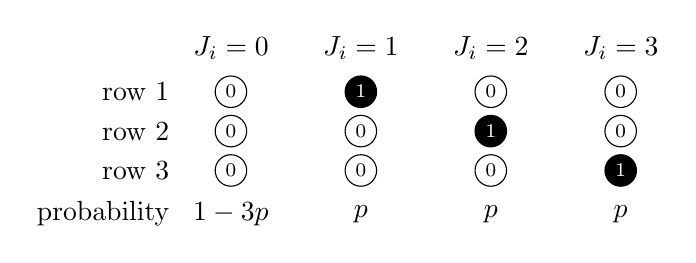
\begin{tikzpicture}[x=1.65cm,y=0.5cm,
  bit/.style={circle,draw,minimum size=4mm,inner sep=0pt},
  present/.style={bit,fill=black,text=white}]
  \foreach \x/\y in {0/1,0/2,0/3,1/1,1/2,2/1,2/3,3/2,3/3}
    \node[bit] at (\x,\y) {\scriptsize 0};
  \foreach \x/\y in {1/3,2/2,3/1}
    \node[present] at (\x,\y) {\scriptsize 1};
  \node at (0,4.1) {$J_i=0$};
  \node at (1,4.1) {$J_i=1$};
  \node at (2,4.1) {$J_i=2$};
  \node at (3,4.1) {$J_i=3$};
  \node at (0,-0.1) {$1-3p$};
  \foreach \x in {1,2,3} {\node at (\x,-0.1) {$p$};}
  \node[anchor=east] at (-0.4,3) {row 1};
  \node[anchor=east] at (-0.4,2) {row 2};
  \node[anchor=east] at (-0.4,1) {row 3};
  \node[anchor=east] at (-0.4,-0.1) {probability};
\end{tikzpicture}
\caption{One coordinate of the sparse coupling, illustrated with three
rows and $3p<1$. Each row contains this coordinate with probability $p$;
the union contains it with probability $3p$. Making these choices
independently across coordinates gives the required product laws.}
\label{fig:coupling}
\end{figure}

\step{Step 1.3 (the family of $L$-fold unions is likely at density $q$).}
Define
\[
\mathcal F
=\{D_1\cup\cdots\cup D_L:D_1,\ldots,D_L\in\mathcal D\}.
\]
On the event in~\eqref{eq:all-good-rows}, $R=R_1\cup\cdots\cup R_L$
belongs to $\mathcal F$. Since $R$ has law $\mu_q$,
\[
\mu_q(\mathcal F)=\mathbb P(R\in\mathcal F)
\ge\frac{31}{32}\ge\frac12.
\]

\step{Step 1.4 (the exceptional families agree).}
A union of $32$ members of $\mathcal F$ is a union of $32L$ members of
$\mathcal D$; conversely, a union of $32L$ members of $\mathcal D$,
grouped into $32$ blocks of $L$, is a union of $32$ members of
$\mathcal F$. So the two collections of unions coincide, and by
\eqref{eq:exceptional-definition}
\[
E_{32}(\mathcal F)=E_{32L}(\mathcal D)=E_k(\mathcal D).
\]

\step{Step 1.5 (conclusion of Case 1).}
By Step~1.3, Proposition~\ref{prop:half-density} applies to $\mathcal F$
at density $q$: $E_{32}(\mathcal F)$ is $(q/L)$-small. Since $q/L=p$ and
$E_{32}(\mathcal F)=E_k(\mathcal D)$, the family $E_k(\mathcal D)$ is
$p$-small.

\medskip
\noindent\emph{Case 2: $Lp\ge1$.}

\step{Step 2.1 (the coupling).}
Set
\[
\theta=\frac{p-1/L}{1-1/L}.
\]
Then $\theta\in[0,1)$: the numerator is nonnegative because $Lp\ge1$, and
smaller than the denominator because $p<1$. At each coordinate $i$,
independently across coordinates, choose a \emph{mandatory row} uniformly
among the $L$ rows; put $i$ into that row, and, conditionally on this
choice, put $i$ into each other row independently with probability
$\theta$. Let $R_j$ be the set of coordinates put into row $j$.

\step{Step 2.2 (laws and union).}
For each fixed $j$ and $i$,
\[
\mathbb P(i\in R_j)
=\frac1L\cdot1+\left(1-\frac1L\right)\theta
=\frac1L+\left(p-\frac1L\right)=p .
\]
The event $\{i\in R_j\}$ depends only on the choices made at coordinate
$i$, and these are independent across coordinates; so $R_j$ has law
$\mu_p$. Every coordinate lies in its mandatory row, so
$R_1\cup\cdots\cup R_L=[N]$ in every outcome.

\step{Step 2.3 (conclusion of Case 2).}
By~\eqref{eq:all-good-rows} the event that all $L$ rows lie in
$\mathcal D$ has positive probability, so some outcome gives
$D_1,\ldots,D_L\in\mathcal D$ with $D_1\cup\cdots\cup D_L=[N]$. Repeating
this tuple $32$ times gives $32L=k$ members of $\mathcal D$ with union
$[N]$, which contains every $S\subseteq[N]$. Hence
$E_k(\mathcal D)=\varnothing$, which the empty family covers at cost $0$
(fact \ref{O:sub}). The boundary case $Lp=1$ is included, with $\theta=0$.
\end{proof}

\section{A consequence, context, and a side result}
\label{sec:context}

Nothing in this section is used in the proof of Theorem~\ref{thm:main}.

\subsection{Positive selector processes}

The connection to positive selector processes
\cite[Section~7]{Talagrand10} gives a concrete consequence of
Theorem~\ref{thm:main}, recovering the positive-selector conclusion proved
by Park and Pham \cite[Theorem~1.2]{ParkPham24}. For a nonempty family
$T\subseteq[0,\infty)^N$, define
\[
\phi(S)=\sup_{t\in T}\sum_{i\in S}t_i,
\qquad M=\mathbb E_{\mu_p}\phi,
\]
and suppose $0<M<\infty$. \emph{Claim:} with $k=2^{75}$, the family
$\{S:\phi(S)\ge k^2M\}$ is $p$-small.

\begin{proof}
Let $\mathcal D=\{D:\phi(D)<kM\}$.
\begin{enumerate}[label=(\arabic*)]
\item Markov's inequality gives
$\mu_p\{\phi\ge kM\}\le M/(kM)=1/k$, so $\mu_p(\mathcal D)\ge1-1/k$.
\item Since all $t_i\ge0$, $\phi$ is monotone ($S\subseteq S'$ implies
$\phi(S)\le\phi(S')$) and subadditive under unions
($\sum_{i\in A\cup B}t_i\le\sum_{i\in A}t_i+\sum_{i\in B}t_i$ for each
$t$, hence $\phi(A\cup B)\le\phi(A)+\phi(B)$).
\item If $S\subseteq D_1\cup\cdots\cup D_k$ with all
$D_j\in\mathcal D$, then by (2)
$\phi(S)\le\sum_j\phi(D_j)<k\cdot kM$. Hence
$\{S:\phi(S)\ge k^2M\}\subseteq E_k(\mathcal D)$.
\item By (1) and Theorem~\ref{thm:main}, $E_k(\mathcal D)$ is $p$-small,
and a cover of it covers the subfamily in (3) (fact \ref{O:sub}).
\qedhere
\end{enumerate}
\end{proof}

Thus the large-value event has explicit containment witnesses, beyond the
small probability already supplied by Markov's inequality.

\subsection{Context and related work}

\paragraph{Origin of the problem.}
The name reflects the analogy with Talagrand's Gaussian convexity
question~\cite[Conjecture~2.1]{Talagrand10}: can a bounded number of
sums of a compact balanced set of sufficiently large Gaussian measure
contain a convex set of Gaussian measure at least $1/2$, uniformly in
the dimension? (Balanced means closed under multiplication by scalars of
absolute value at most one.) In the discrete problem, unions replace sums,
and containment covers describe the exceptional sets. Talagrand formulated
the discrete-convexity conjecture in \cite[Conjecture~7.1]{Talagrand10}: a
fixed number of members of a sufficiently likely family should cover every
set outside a $p$-small exceptional family. The same original-density
formulation appears as Research Problem~13.3.2 in~\cite{Talagrand21}, whose
Proposition~13.3.3 explains its connection to positive selector processes.
Theorem~\ref{thm:main} proves this conjecture.

\paragraph{Related developments.}
Hua, Song, and Tudose resolve Talagrand's Gaussian convexity problem and
derive a discrete conclusion with three unions and covering density
$p^C$, for a universal constant $C$, when the starting family is
sufficiently likely~\cite[Corollaries~1.3--1.4]{HuaSongTudose26}.
Ascoli, He, Park, and Talagrand give a threshold reformulation of discrete
convexity and prove cases for several graph-containment
properties~\cite[Proposition~1.5 and Theorems~1.10--1.13]{AscoliEtAl26}.

There is also a fractional version of smallness: a \emph{fractional
cover} of $\mathcal A$ of cost at most $1/2$ at density $p$ is an
assignment of nonnegative coefficients $a_I$ with
\[
\sum_{I\subseteq S}a_I\ge1\quad(S\in\mathcal A),
\qquad
\sum_{I\subseteq[N]}p^{|I|}a_I\le\frac12.
\]
Talagrand introduced this relaxation alongside integral
smallness~\cite[Sections~6 and~7]{Talagrand10}.
Li resolves the fractional discrete-convexity problem through a quantitative
obstruction to probability measures whose containment probabilities
are bounded by $p^{|I|}$~\cite[Theorem~1.9]{Li26}.
Combining fractional information with rounding, Park obtains an integral
cover of $E_2(\mathcal D)$ at density
$p/(C\max\{1,\log\log(1/p)\})$
whenever $\mu_p(\mathcal D)>1/2$, for a universal
$C$~\cite[Corollary~3.5]{Park26}.

\paragraph{Antecedents of the method.}
With two rows instead of $32$, the signed column mass $\widetilde P$ of
Lemma~\ref{lem:exceptional} is Li's signed kernel after multiplication by
the Bernoulli masses~\cite[Section~2]{Li26}. Park also notes the
extension of Li's argument to an even number of unions
\cite[Corollary~3.5, footnote~3]{Park26}. What is new here is the
combination of the higher powers obtained from $32$ rows with
Lemma~\ref{lem:covering}, which yields a fixed density loss. The
signed-operator approach to forbidden configurations and its biased
Fourier basis have earlier forms in Friedgut~\cite[Section~2.2]{Friedgut08}
and Ellis, Filmus, and
Friedgut~\cite[Sections~2.2 and~4.1]{EllisFilmusFriedgut12}. Unions of
sampled edges also appear in the covering constructions of Fischer and
Person~\cite[Sections~1.1 and~2]{FischerPerson25};
Lemma~\ref{lem:covering} is proved in full above.

\subsection{Two unions at constant density loss}

Combining Li's result with the companion constant-factor rounding theorem
gives the following two-union tradeoff. Compared with
Theorem~\ref{thm:main}, it uses only two unions and a weaker measure
hypothesis, but concludes smallness only at the lower density $p/C$ (a
weaker conclusion, by fact \ref{O:mono}).

\begin{corollary}[Two unions at constant density loss]
\label{cor:two-union}
There is a universal constant $C\ge1$ such that, for every integer $N\ge1$,
every $p\in(0,1)$, and every family $\mathcal D\subseteq2^{[N]}$,
\[
\mu_p(\mathcal D)>\frac12
\quad\Longrightarrow\quad
E_2(\mathcal D)\text{ is }(p/C)\text{-small}.
\]
\end{corollary}

\emph{Status of the proof.} Unlike the rest of this paper, the proof is a
chain of external results. The statements (i) and (iii) below are quoted
exactly as the source uses them; this rewrite does not reprove them and has
not compared them with the cited papers. Only the glue between them is
checked here.

\begin{proof}
If $E_2(\mathcal D)=\varnothing$, the empty cover suffices. Otherwise:
\begin{enumerate}[label=(\roman*)]
\item \emph{$E_2(\mathcal D)$ is a nonempty proper increasing family.}
Since $\mu_p(\mathcal D)>1/2$, $\mathcal D\ne\varnothing$, so
$\varnothing\subseteq D\cup D$ for some $D\in\mathcal D$ and
$\varnothing\notin E_2(\mathcal D)$. If $S\in E_2(\mathcal D)$ and
$S\subseteq S'$, then $S'$ is contained in no $D_1\cup D_2$ either. By
Li's result \cite[Corollary~3.1]{Li26} in Park's fractional-cover
formulation \cite[Theorem~3.4]{Park26}, this family has a fractional cover
of cost at most $1/2$ at density $p_1=p/2$.
\item \emph{Capping.} Replace each coefficient $a_I$ by $\min\{a_I,1\}$.
Coverage is preserved: if some $I\subseteq S$ had $a_I\ge1$, the capped
coefficient alone is $1$; otherwise nothing changed for $S$. The cost does
not increase.
\item \emph{Rounding.} The companion expectation-threshold
theorem~\cite[Theorem~1.1]{OpenAIThreshold26} then gives an integral cover
of cost at most $1/2$ at density $p_1/(25\cdot512^4)$.
\end{enumerate}
Since $p_1/(25\cdot512^4)=p/(50\cdot512^4)$, the constant
$C=50\cdot512^4$ suffices.
\end{proof}

\begin{remark}[Consistency check for input (i); not part of the source's
proof]
The conclusion quoted in (i) can be confirmed with the tools of
Section~\ref{sec:weights}, taking $q=p$, $\mathcal F=\mathcal D$ and
$\mu=\mu_p(\mathcal D)>1/2$. The proof of Lemma~\ref{lem:exceptional}
runs verbatim with $2$ rows in place of $32$ and gives
$0=\sum_{U\subseteq S}(-1)^{|U|}b(U)^2$ for $S\in E_2(\mathcal D)$, hence
$\sum_{\varnothing\ne U\subseteq S}w(U)\ge b(\varnothing)^2=\mu^2$. By
\eqref{eq:fhat-b} and \eqref{eq:parseval},
$\sum_{U}(p/(1-p))^{|U|}w(U)=\mu$, so
$\sum_{U\ne\varnothing}p^{|U|}w(U)\le\mu-\mu^2$. Thus
$a_U=w(U)/\mu^2$ ($U\ne\varnothing$) is a fractional cover of
$E_2(\mathcal D)$ whose cost at density $p/2$ is at most
$\tfrac12(\mu-\mu^2)/\mu^2=(1-\mu)/(2\mu)<1/2$.
\end{remark}

\section{Verification checklist}
\label{sec:checklist}

No step of the chain leading to Theorem~\ref{thm:main} is marked
unverified. The steps that carry the weight, in the order a sceptical
reader might check them:

\begin{enumerate}[label=\arabic*.]
\item \textbf{The signed identity}
$0=\sum_{U\subseteq S}(-1)^{|U|}b(U)^{32}$
(Lemma~\ref{lem:exceptional}). Check that $\widetilde P$ vanishes on the
all-zero column \eqref{eq:zero-column}, that this forces every term of
\eqref{eq:vanishing} to vanish (Step~2), and that each expanded term
factors over the $32$ rows with row factor exactly $b(U)$, including the
split $(1-q)^{32|U|}=\prod_j(1-q)^{|U|}$ (Steps~3--4).
\item \textbf{The normalization}
$\widehat f(U)=(q/(1-q))^{|U|/2}b(U)$, equation \eqref{eq:fhat-b}
(Lemma~\ref{lem:global}, Step~2). It is what turns Parseval into
$\sum_Uq^{|U|}w(U)\le1$ with the factor $q^{|U|}$, not a smaller one.
\item \textbf{The extension bound} \eqref{eq:covering-extension}
(Lemma~\ref{lem:covering}, Step~3) and its two uses: with $B=e$ for the
pair cost \eqref{eq:covering-pair-cost}, and with $B$ a prefix union for
$W_{n+1}\le\tau(1+rm)^rW_n$ (Step~6).
\item \textbf{The survival probability and numerics} in
Lemma~\ref{lem:covering}, Steps~7--8: the $m^2$ pair indices of a tuple of
distinct edges are distinct (so independence applies), and
$4h+13rh+1\le2^{6h}=\pi m$.
\item \textbf{The binning arithmetic} in the proof of
Proposition~\ref{prop:half-density}: $h\ge64r$ for occupied bins
(Step~2(ii)), the hypothesis $|\mathcal H_{r,h}|\rho^r\le2^{h+1}$ of the
covering lemma (Step~2(iii)), and the two geometric sums
\eqref{eq:bin-cost-sum} and \eqref{eq:bin-power-sum}, in particular
$\frac{16}{15(2^{256}-1)}<2^{-32}$.
\item \textbf{The coupling} in the proof of Theorem~\ref{thm:main}: each
row has law exactly $\mu_p$ and the union has law exactly $\mu_{Lp}$
(Step~1.2), respectively is $[N]$ (Step~2.2, including
$\tfrac1L+(1-\tfrac1L)\theta=p$); the identity
$E_{32}(\mathcal F)=E_k(\mathcal D)$ (Step~1.4); and the constants
$k=32L$, $1-L/k=31/32$.
\item \textbf{External inputs.} The main chain uses only Parseval's
identity. Corollary~\ref{cor:two-union} alone depends on three cited
results, quoted but not reproved here; see the status note before its
proof.
\end{enumerate}

\begin{thebibliography}{99}

\bibitem{AscoliEtAl26}
Ruben Ascoli, Xiaoyu He, Jinyoung Park, and Michel Talagrand,
\emph{A reformulation of the discrete Convexity Conjecture via
$k$-thresholds},
arXiv:2608.11183v1, 2026.
\href{https://arxiv.org/abs/2608.11183v1}{arXiv:2608.11183v1}.

\bibitem{EllisFilmusFriedgut12}
David Ellis, Yuval Filmus, and Ehud Friedgut,
\emph{Triangle-intersecting families of graphs},
Journal of the European Mathematical Society \textbf{14} (2012),
no.~3, 841--885.
\href{https://doi.org/10.4171/JEMS/320}{doi:10.4171/JEMS/320}.

\bibitem{FischerPerson25}
Thomas Fischer and Yury Person,
\emph{Further remarks on fractional vs. expectation thresholds},
arXiv:2505.21782v1, 2025.
\href{https://doi.org/10.48550/arXiv.2505.21782}{doi:10.48550/arXiv.2505.21782}.

\bibitem{Friedgut08}
Ehud Friedgut,
\emph{On the measure of intersecting families, uniqueness and stability},
Combinatorica \textbf{28} (2008), no.~5, 503--528.
\href{https://doi.org/10.1007/s00493-008-2318-9}{doi:10.1007/s00493-008-2318-9}.

\bibitem{HuaSongTudose26}
Dongming (Merrick) Hua, Antoine Song, and Stefan Tudose,
\emph{On Talagrand's Convexity Conjecture},
arXiv:2605.10908v2, 2026.
\href{https://arxiv.org/abs/2605.10908v2}{arXiv:2605.10908v2}.

\bibitem{Li26}
Chen Li,
\emph{On $p$-spread measures},
arXiv:2609.08967v1, 2026.
\href{https://arxiv.org/abs/2609.08967v1}{arXiv:2609.08967v1}.

\bibitem{ODonnell14}
Ryan O'Donnell,
\emph{Analysis of Boolean Functions},
Cambridge University Press, Cambridge, 2014.
Author's corrected text, 2021:
\href{https://arxiv.org/abs/2105.10386v1}{arXiv:2105.10386v1}.

\bibitem{OpenAIThreshold26}
OpenAI,
\emph{Integral and fractional expectation thresholds are equivalent},
OpenAI Math Release preprint
\href{https://github.com/openai/math/blob/main/preprints/Integral-and-fractional-expectation-thresholds-are-equivalent-September-23-2026/paper.pdf}{OAI:Integral-and-fractional-expectation-thresholds-are-equivalent-September-23-2026},
2026.

\bibitem{Park26}
Jinyoung Park,
\emph{A dimension-free comparison between expectation thresholds and
fractional expectation thresholds},
arXiv:2609.14681v1, 2026.
\href{https://arxiv.org/abs/2609.14681v1}{arXiv:2609.14681v1}.

\bibitem{ParkPham24}
Jinyoung Park and Huy Tuan Pham,
\emph{On a conjecture of Talagrand on selector processes and a consequence
on positive empirical processes},
Annals of Mathematics \textbf{199} (2024), no.~3, 1293--1321.
\href{https://doi.org/10.4007/annals.2024.199.3.6}{doi:10.4007/annals.2024.199.3.6}.

\bibitem{Talagrand10}
Michel Talagrand,
\emph{Are many small sets explicitly small?},
Proceedings of the Forty-Second ACM Symposium on Theory of Computing,
ACM, New York, 2010, 13--36.
\href{https://doi.org/10.1145/1806689.1806693}{doi:10.1145/1806689.1806693}.

\bibitem{Talagrand21}
Michel Talagrand,
\emph{Upper and Lower Bounds for Stochastic Processes:
Decomposition Theorems},
2nd ed., Ergebnisse der Mathematik und ihrer Grenzgebiete, 3.~Folge,
vol.~60, Springer, Cham, 2021.
\href{https://doi.org/10.1007/978-3-030-82595-9}{doi:10.1007/978-3-030-82595-9}.

\end{thebibliography}

\end{document}
